\documentclass[10pt, a4paper]{scrartcl}

\usepackage[utf8]{inputenc}
\usepackage[ngerman]{babel}
\usepackage{amsmath}
\usepackage{mathtools}
\usepackage{amsfonts}
\usepackage{hyperref}
\usepackage{graphicx}

\title{Deep learning lab for autonomous driving \\ Report for ex. sheet 1}
\author{Michael Floßmann -- 4348852}

\date{2018--05--04}

\begin{document}
% \maketitle

\section{Report for exercise Sheet 1 of the deep learning lab for autonomous driving}
Author: Michael Floßmann -- 4348852
\section{Introduction}
In this exercise, we were supposed to use the GTSRB dataset to train a
convolutional network, to recocnize street signs.

\section{Structure of the CNN}
The basic structure of the CNN is depicted in table \ref{tab:net}.
\begin{table}[!htbp]
  \centering
  \begin{tabular}{lcccc}
    &Conv1&Max-pool1&Conv2d&Max-pool2\\ \hline
    Kernel size & 3 & 2 & 3 & 2 \\
    Input depth & 3 & & 30 & \\
    Output depth & 30 & & 60 & \\
    Padding & 1 & 0 & 0 & 0 \\
    Stride & 1 & 2 & 1 & 0 \\
  \end{tabular}
  \label{tab:net}
  \caption{Structure of the CNN}
\end{table}

After this, a dropout filter is applied and after linearizing the data, it's
first brought to a size of $512\times 1$ and then to $43\times 1$ by linear
layers. In the end, a softmax filter is applied.

Every activation layer is a ReLU-Function.

\subsection{Sampling}
For sampling, the Training dataset was shuffled and split into an
Training-Validation fraction of 80/20.

\subsection{Optimization}
The optimizer is a stochastic gradient descent optimizer with momentum of 0.5
and varying learning rates.

Because the deadline grew closer, 10 epochs were performed, although the data
suggested that overfitting didn't begin yet.

\section{Results}
\begin{figure}[!htbp]
  \centering
  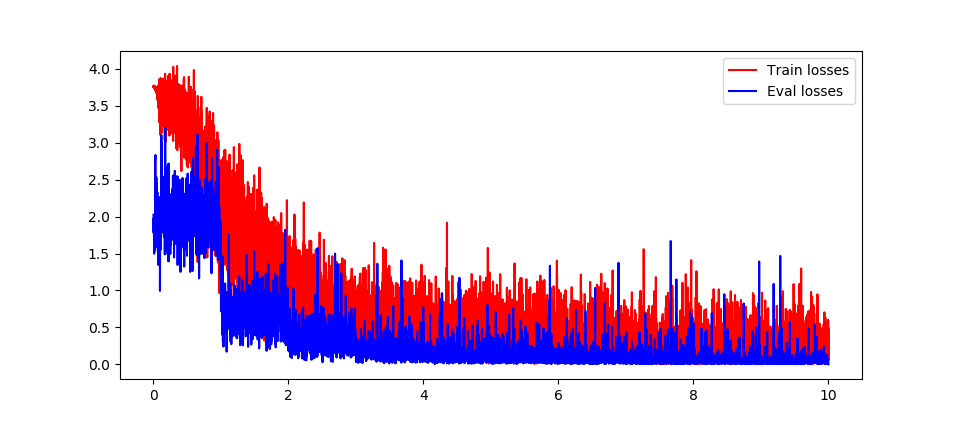
\includegraphics[width=0.5\textwidth]{lr_0_01.png}
  \caption{Learn rate: 0.01, Accuracy: TBD}
  \label{fig:lr_0.01}
\end{figure}

\begin{figure}[!htbp]
  \centering
  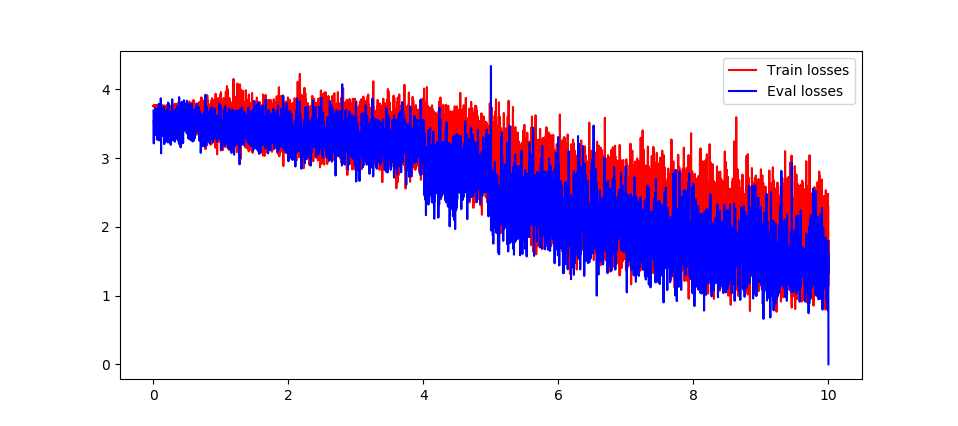
\includegraphics[width=0.5\textwidth]{lr_0_001.png}
  \caption{Learn rate: 0.001, Accuracy: TBD}
  \label{fig:lr_0.001}
\end{figure}

\begin{figure}[!htbp]
  \centering
  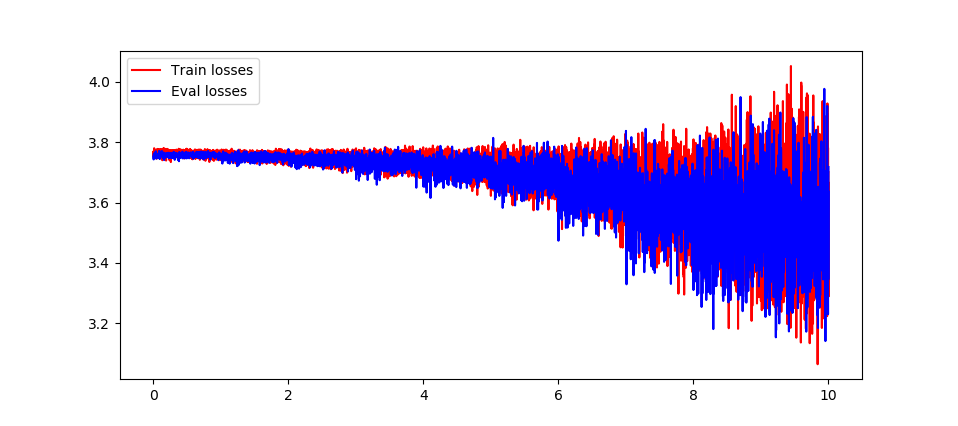
\includegraphics[width=0.5\textwidth]{lr_0_0001.png}
  \caption{Learn rate: 0.0001, Accuracy: TBD}
  \label{fig:lr_0.001}
\end{figure}

\subsection{Performance on the training set}
The best model on the validation set performed with an accuracy of TBD\% on the
test set.


\end{document}